\scanpage{18}
Ceci dit, une décomposition cellulaire $\mathcal P$ de $X$ est dite $F$-\uline{régulière} si \deleted{les feuilles sont $\unsure{\in F_r}$}\inserted{$F_{\mathcal P}$ muni de la notion de \uline{régularité} induite par $F,F_r$ satisfait la condition $\unsure{S|B}$, i.e. \deleted{$\unsure{\mathcal P}$} \unsure{plus précisément} $\forall\deleted{\unsure{X}}Y$ fermé $\mathcal P$-saturé $Y_s$ est $\mathcal P$-saturé. (\uline{Ceci implique que les feuilles sont} $\in F_r$)}

\uline{Prop.} Sous les conditions a) b) c) d) \unsure{e)} \deleted{\unsure{f)}} sur $F$, et la condition $(\unsure{S|B})$ sur $F_r\subset F$, si $\Phi\subset F$ est une partie finie, il existe une partition $F$-\uline{régulière} de $X$, et \unsure{$=$|---} une plus \uline{grossière} telle partition. Si $F$ satisfait \unsure{$=$|---} f), alors il existe une partition $F$-\uline{régulière} de $X$ à feuilles connexes, et une plus \uline{grossière} telle.
\figure{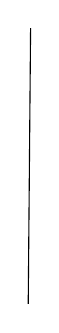
\begin{tikzpicture}[x=1cm,y=1cm]\draw (0,0)--(0.03,3.5);\end{tikzpicture}}

\inserted{QPS $\Phi$ stable par $\unsure{\complement}$ .}
Soit
\[
X'=\bigcup_{Y\in\Phi}\dot Y\cup\mathring Y_{\mathrm{sing}},\qquad U=X-X'.
\]
Les $Y\cap U$ sont ouverts et fermés, et \uline{réguliers}. On continue comme plus haut, \inserted{avec les $U_i$, mais dans $\Phi'$ on met aussi les $(\overline{U_i})_{\mathrm{sing}}$} Dans le cas où $F$ satisfait d), on passe encore \inserted{avant} aux composantes connexes des $U_i$.

\inserted{\uline{Cor. 1}} Donc $F$ est réunion filtrante de $F_{\mathcal P}$ où $\mathcal P$ est à feuilles $F$-\uline{régulières} (resp. $F$-\uline{régulières} et connexes, si $F$ satisfait d)).

\uline{Cor 2} Sup \inserted{finis} dans les partitions $F$-\uline{régulières} (resp. à fibres connexes)

\uline{Cor 3} Partition $F$-régulière canonique de $X$
\mspage{19}
